\subsubsection{Smartwatch introduction}
\label{subsec:sw2}
The smartwatch that was chosen to do the project with is the Sony 
Smartwatch 2. It is a cheap watch and it is programmable. The SDK has recently been updated and is easy to use. We have used the SDK to quickly make an application. There are many examples which are easily installed. These examples were used to generate traffic for the Ubertooth to detect. This sped up the process of finding targeting and decoding the packets. 
\begin{figure}[!h]
  \begin{center}
	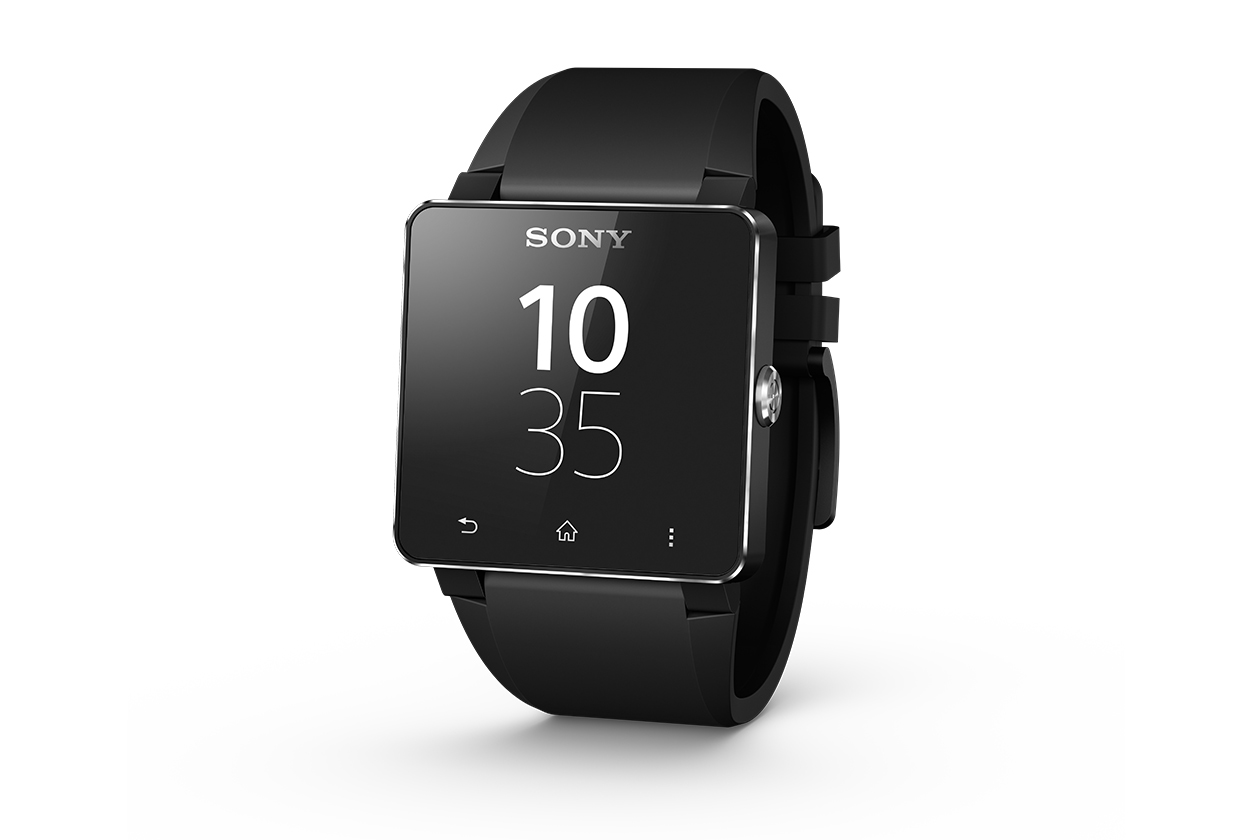
\includegraphics[width=200px]{images/sw2.jpg}
	\label{Sony Smartwatch 2}
  \end{center}
\end{figure}
\\
All the Sony devices use an application called Smart Connect. This application keeps track of all the devices that want to make contact with the phone. It also keeps track of the applications that are installed on the watch. Whenever the pairing is stopped between the phone and the watch all the previous installed applications are removed from the watch until they are paired again/
\subsubsection{Smartwatch applications}
\label{subsubsec:sw_app}
%needs revision
The life cycle of a smartwatch app is about the same as an application on a phone or tablet. The thing with smartwatch apps is they only work when connected to another device. When you stop the connection with your smartwatch the apps will disappear from the watch. What you do is open smart connect on your "master device" and install the applications you want to use on your watch. The app needs to be registered first before it will show up. The smartwatch can start apps on the phone from. All information and changes done to the app are first relayed to the master device the calculation is done and then send back to the smartwatch. The smartwatch keeps polling and for new information from the the master device. 